\documentclass[11pt]{beamer}

\usetheme{Oxygen}
\usepackage{thumbpdf}
\usepackage{wasysym}
\usepackage{ucs}
\usepackage[utf8]{inputenc}
\usepackage{pgf,pgfarrows,pgfnodes,pgfautomata,pgfheaps,pgfshade}
\usepackage{verbatim}
\usepackage{anyfontsize}
\usepackage{minted}
\usepackage{graphicx}

\pdfinfo
{
  /Title       (LaTeX)
  /Creator     (TeX)
  /Author      (Miguel Angel Gordian)
}


\title{\LaTeX}
\subtitle{Inicio}
\author{Miguel Angel Gordian}
\date{Marzo 23, 2012}

\begin{document}

\frame{\titlepage}

\section*{}
\begin{frame}
  \frametitle{Resumen}
  \tableofcontents[section=1,hidesubsections]
\end{frame}

\AtBeginSection[]
{
  \frame<handout:0>
  {
    \frametitle{Resumen}
    \tableofcontents[currentsection,hideallsubsections]
  }
}

\AtBeginSubsection[]
{
  \frame<handout:0>
  {
    \frametitle{Resumen}
    \tableofcontents[sectionstyle=show/hide,subsectionstyle=show/shaded/hide]
  }
}

\newcommand<>{\highlighton}[1]{%
  \alt#2{\structure{#1}}{{#1}}
}

\newcommand{\icon}[1]{\pgfimage[height=1em]{#1}}

% configuración de minted
\definecolor{bg}{rgb}{0.85,0.85,0.85}
\usemintedstyle{emacs}

\newminted{tex}{linenos=true, bgcolor=bg}
%%%%%%%%%%%%%%%%%%%%%%%%%%%%%%%%%%%%%%%%%
%%%%%%%%%% Content starts here %%%%%%%%%%
%%%%%%%%%%%%%%%%%%%%%%%%%%%%%%%%%%%%%%%%%


\section{Introducci\'on}

\section*{}
\frame{
  \vfill
  \centering
  \highlighton{
    \usebeamerfont*{frametitle}{\fontsize{50}{1}\selectfont LaTeX}

    \usebeamerfont*{framesubtitle}Definici\'on
  }
  \vfill
}

\begin{frame}
  \frametitle{¿Qu\'e es \LaTeX?}
  %%  \begin{block}{Definición}
  \begin{itemize}
    \item<1-> \LaTeX es un softaware de composici\'on de documentos, en otras palabras
   es un sistema de preparaci\'on de documentos.
    \item<2-> \LaTeX es libre, es software open source.
    \item<3-> Escrito por Leslie Lamport
    \item<4-> Basado en el motor de composici\'on de TeX escrito por  Donald Knuth
  \end{itemize}
%%  \end{block}
\end{frame}


%% \begin{frame}
%%   \frametitle{En pocas palabras}
%%   \vfill
%%   \begin{center}
%%     $ \begin{array}{1}
%%     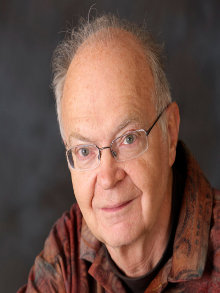
\includegraphics[width=2.5cm, heigth=2.5cm]{imagenes/Donald-Knuth} 
%%     \end{array}
%%     $ {\fontsize{30}{1}\selectfont +} $ 
%%     \begin{array}{1}
%%        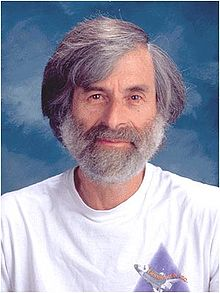
\includegraphics[width=2.5cm, heigth=2.5cm]{imagenes/Leslie-Lamport}
%%     \end{array} 
%%     $ {\fontsize{30}{1}\selectfont = \LaTeX}
%%   \end{center}
%%   \vfill
%% \end{frame}

\begin{frame}
  \frametitle{Beneficios}
  
  \begin{itemize}
    \item<1-> \LaTeX  esta especialmente provisto para documentos cientificos y tecnicos.
    \item<2-> Niveles de referencia cruzada, su
      numeración automatica y  generaci\'on de listas de contenido, figuras,
      tablas, indices, glosarios y bibliograf\'ia.
    \item<3-> Gran cantidad de templates para cartas, presentaciones, 
      partituras, y notaciones para juegos. 
  \end{itemize}
  \begin{equation}
    \sum_{i=1}^n i^2 = \frac{n \times (n+1) \times (2n+1)}{6}
  \end{equation}
\end{frame}


\section{Primeros pasos}
\begin{frame}[fragile]
  \frametitle{Primer paso}
  \framesubtitle{Hola mundo en \LaTeX}
  \begin{texcode}
% Hola mundo en LaTeX
\documentclass[a4paper, 13pt]{article}

\begin{document}
\title{Hola mundo}
\author{Miguel Angel Gordi\'an}
\date{Marzo 23, 2012}
\maketitle

\section{saluda}
Hola mundo en \LaTeX

\end{document}
  \end{texcode}
\end{frame}


\begin{frame}[fragile]
  \frametitle{Compilando}
  \usemintedstyle{tango}
  \begin{itemize}
    \item pdf: \mint[bgcolor=bg]{sh}/ $ pdflatex hola.tex/
      \vfill
    \item dvi: \mint[bgcolor=bg]{sh}/ $ latex hola.tex/
  \end{itemize}
\end{frame}


%% \begin{frame}
%%   \frametitle{Segundo Paso}
%%   \framesubtitle{Disecci\' on}
%%   \begin{itemize}
%%   \item \textit{\textbf{$\backslash$documenclass}}:
%%   \item \textit{\textbf{$\backslash$begin y $\backslash$end}}:
%%   \item \textit{\textbf{$\backslash$LaTeX}}:
%%   \end{itemize}
%% \end{frame}


\frame{
  \vspace{2cm}
  {\huge ¿Preguntas?}

  \vspace{3cm}
  \begin{flushright}
    Miguel Angel Gordian

    \structure{\footnotesize{os.aioria@gmail.com}}
  \end{flushright}
}

\end{document}
